% Sept-26 draft -- starter deck, no content yet
% UIUC SRSE 2026, September 26, 2026
% Build: pdflatex 2026-09-26-draft.tex  (run twice)

\documentclass[aspectratio=169,10pt]{beamer}

\usepackage[T1]{fontenc}
\usepackage[utf8]{inputenc}
\usepackage[sfdefault]{FiraSans}
\usepackage[scaled=0.85]{FiraMono}
\usepackage{listings}
\usepackage{tikz}
\usepackage{tcolorbox}
\usepackage{booktabs}
\usepackage{graphicx}
\usepackage{stmaryrd}

\usetheme{metropolis}
\metroset{sectionpage=progressbar, numbering=fraction, progressbar=frametitle}

\usetikzlibrary{arrows.meta, positioning, calc, fit, backgrounds}
\tcbuselibrary{skins}

% Palette
\definecolor{lgInk}{HTML}{23373B}
\definecolor{lgAccent}{HTML}{C25E00}
\definecolor{lgTeal}{HTML}{0F7B8A}
\definecolor{lgRed}{HTML}{B3282D}
\definecolor{lgGreen}{HTML}{2E7D32}
\definecolor{lgGrey}{HTML}{6B7A7D}
\definecolor{lgWash}{HTML}{F2F4F4}
\definecolor{lgWashWarm}{HTML}{FBF1E6}

\setbeamercolor{normal text}{fg=lgInk}
\setbeamercolor{frametitle}{bg=lgInk, fg=white}
\setbeamercolor{progress bar}{fg=lgAccent}
\setbeamercolor{alerted text}{fg=lgAccent}

% Code listings
\lstdefinestyle{verus}{
  basicstyle=\ttfamily\scriptsize\color{lgInk},
  keywordstyle=\color{lgTeal}\bfseries,
  morekeywords={ensures,requires,invariant,decreases,proof,assert,spec,fn,let,ghost,loop,while,if,else,use,pub,result},
  showstringspaces=false,
  breaklines=false,
  columns=fullflexible,
  keepspaces=true,
  aboveskip=1pt, belowskip=1pt,
}
\lstset{style=verus}

% Inline helpers
\newcommand{\code}[1]{{\ttfamily #1}}
\newcommand{\hd}[1]{\textbf{\color{lgTeal}#1}}
\newcommand{\good}[1]{{\color{lgGreen}#1}}
\newcommand{\bad}[1]{{\color{lgRed}#1}}

% Boxes
\newtcolorbox{callout}[1][lgAccent]{
  enhanced, colback=lgWashWarm, colframe=#1,
  boxrule=0.1pt, leftrule=2.5pt, arc=1.5pt,
  left=6pt, right=6pt, top=4pt, bottom=4pt, boxsep=0pt,
}

\newtcolorbox{codebox}[2][lgGrey]{
  enhanced, colback=lgWash, colframe=#1,
  boxrule=0.1pt, leftrule=2.5pt, arc=1.5pt,
  left=6pt, right=4pt, top=3pt, bottom=3pt, boxsep=0pt,
  title={\scriptsize\bfseries\color{#1}#2},
  fonttitle=\bfseries, coltitle=#1,
  colbacktitle=lgWash, titlerule=0pt,
  attach title to upper={\par\vspace{1pt}},
}

% TikZ styles
\tikzset{
  stage/.style={
    draw=lgInk, line width=0.7pt, rounded corners=2pt,
    fill=white, inner sep=5pt, align=center,
    font=\scriptsize, text=lgInk, minimum height=9mm
  },
  okstage/.style={stage, draw=lgGreen, fill=lgGreen!8, text=lgGreen},
  mem/.style={stage, draw=lgTeal, fill=lgTeal!8, text=lgTeal},
  flow/.style={-{Stealth[length=2mm]}, line width=0.7pt, draw=lgInk},
  lbl/.style={font=\tiny\itshape, text=lgGrey, inner sep=2pt},
}

% Title
\title{Rust, CUDA and Verus}
\subtitle{A PoC on Rust-CUDA Verifiable Kernels}
\date{October 6, 2026}
\author{Mahadi Hasan \and Anamul Hoque Emtiaj}
\institute{UIUC SRSE 2026}

\begin{document}

\maketitle

% =====================================================================
\begin{frame}{From PyTorch to Rust}

{\scriptsize
\hd{Source of the CUDA kernels:} KernelBench Level~1 tasks (for now).
}

\vspace{10pt}
\begin{center}
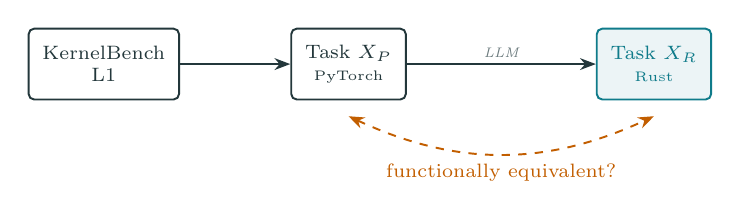
\begin{tikzpicture}[node distance=14mm]
  \node[stage] (kb) {KernelBench\\L1};
  \node[stage, right=of kb] (xp) {Task $X_P$\\\tiny PyTorch};
  \node[mem, right=24mm of xp] (xr) {Task $X_R$\\\tiny Rust};
  \draw[flow] (kb) -- (xp);
  \draw[flow] (xp) -- node[lbl, above] {LLM} (xr);
  \draw[{Stealth[length=2mm]}-{Stealth[length=2mm]}, line width=0.7pt, draw=lgAccent, dashed]
    ([yshift=-2mm]xp.south) to[bend right=25]
    node[font=\scriptsize, text=lgAccent, below] {functionally equivalent?}
    ([yshift=-2mm]xr.south);
\end{tikzpicture}
\end{center}

\vspace{4pt}
\begin{callout}[lgAccent]
\scriptsize
\textbf{Goal.} Guarantee that the translated task computes the same function as the original.
\[
  X_P, X_R : \mathcal{X} \to \mathcal{Y}
  \qquad\qquad
  \forall\, x \in \mathcal{X}.\;\; \llbracket X_P \rrbracket(x) \;=\; \llbracket X_R \rrbracket(x)
\]
\end{callout}

\end{frame}

% =====================================================================
\begin{frame}[fragile]{Two KernelBench L1 tasks}

\begin{columns}[T]
\begin{column}{0.48\textwidth}
\begin{codebox}{19\_ReLU.py}
\begin{lstlisting}[language=Python, basicstyle=\ttfamily\tiny\color{lgInk}]
class Model(nn.Module):
    def __init__(self):
        super(Model, self).__init__()
    def forward(self, x: torch.Tensor) -> torch.Tensor:
        return torch.relu(x)

batch_size = 4096
dim = 393216
def get_inputs():
    x = torch.rand(batch_size, dim)
    return [x]
def get_init_inputs():
    return []
\end{lstlisting}
\end{codebox}

\vspace{2pt}
{\scriptsize
\hd{What it computes.} Replaces every negative entry with zero; the shape is unchanged.
\par\vspace{3pt}\centerline{$x \in \mathbb{R}^{4096 \times 393216}, \qquad y_{ij} = \max(0,\, x_{ij})$}
}
\end{column}

\begin{column}{0.48\textwidth}
\begin{codebox}{47\_Sum\_reduction\_over\_a\_dimension.py}
\begin{lstlisting}[language=Python, basicstyle=\ttfamily\tiny\color{lgInk}]
class Model(nn.Module):
    def __init__(self, dim: int):
        super(Model, self).__init__()
        self.dim = dim
    def forward(self, x: torch.Tensor) -> torch.Tensor:
        return torch.sum(x, dim=self.dim, keepdim=True)

batch_size = 128
dim1 = 4096
dim2 = 4095
reduce_dim = 1
def get_inputs():
    x = torch.rand(batch_size, dim1, dim2)
    return [x]
def get_init_inputs():
    return [reduce_dim]
\end{lstlisting}
\end{codebox}

\vspace{2pt}
{\scriptsize
\hd{What it computes.} Adds up the entries along the middle axis, keeping it as size 1.
\par\vspace{3pt}\centerline{$x \in \mathbb{R}^{128 \times 4096 \times 4095}, \qquad y_{b,0,k} = \sum_{j=0}^{4095} x_{b,j,k}$}
}
\end{column}
\end{columns}

\vfill
{\tiny\color{lgGrey} Source: KernelBench @ \code{423217d}, \code{KernelBench/level1/}; docstrings and imports omitted.}

\end{frame}

% =====================================================================
\begin{frame}[fragile]{Faithful spec extraction}

{\scriptsize
Initially, Mahadi worked on how to \emph{faithfully} extract a specification from a PyTorch source.
The Python file \emph{is} the specification, so the job is \textbf{denotation}: what function does it compute?
}

\vspace{4pt}
\begin{codebox}{Task 47 (PyTorch)}
\begin{lstlisting}[language=Python, basicstyle=\ttfamily\tiny\color{lgInk}]
return torch.sum(x, dim=1, keepdim=True)
\end{lstlisting}
\end{codebox}

\vspace{2pt}
{\scriptsize
\newcommand{\qn}[1]{\tikz[baseline=(n.base)]\node[circle, fill=lgTeal, text=white, inner sep=1pt, font=\tiny\bfseries] (n) {#1};}
\newcommand{\spec}[1]{\colorbox{lgWash}{\ttfamily\tiny\frenchspacing #1}}
\renewcommand{\arraystretch}{1.35}
\begin{tabular}{@{}p{0.38\textwidth}@{\hspace{6pt}}c@{\hspace{6pt}}l@{}}
\multicolumn{1}{@{}l}{\hd{Question about I/O}} & & \hd{Spec it creates} \\
\qn{1} How is the input \code{x} held?
  & $\Rightarrow$ & \spec{x: Seq<i32>, rows: int, cols: int\quad// flat, row-major} \\
\qn{2} Which inputs feed output cell \code{r}?
  & $\Rightarrow$ & \spec{row(x, r, cols) = x.subrange(r*cols, r*cols + cols)} \\
\qn{3} What is done with them?
  & $\Rightarrow$ & \spec{fold\_sum(s) = if s.len() == 0 \{ 0 \} else \{ s[0] + fold\_sum(s.skip(1)) \}} \\
\qn{4} What type is an output value?
  & $\Rightarrow$ & \spec{fold\_sum(s: Seq<i32>) -> int\quad// overflow cannot hide in the spec} \\
\qn{5} How many outputs, and what is each?
  & $\Rightarrow$ & \spec{torch\_sum\_dim1(x, rows, cols) = Seq::new(rows, |r| fold\_sum(row(x, r, cols)))} \\
\end{tabular}
}

\vspace{4pt}
\begin{callout}[lgAccent]
\scriptsize\raggedright
\textbf{Insights.} Questions about I/O reveal the necessary specs.
However, faithfulness up to this point remains a spec-testing problem; human audit remains the final standard.
\end{callout}

\vfill
{\tiny\color{lgGrey} Source: \code{deliverables/2026-09-18/example.md}.}

\end{frame}

% =====================================================================
% Anamul's section (pages 5--8, 10--11): helpers
% Colour roles, used the same way on every slide of this section:
%   human = lgAccent, builder agent = lgInk, reviewer agent = lgTeal,
%   automatic gate / pass = lgGreen, fail / send back = lgRed (dashed)
\newcommand{\byanamul}{\enspace{\mdseries\color{white!72!lgInk}(Anamul)}}
\newcommand{\anum}[2][lgInk]{\tikz[baseline=(n.base)]\node[circle, fill=#1, text=white, inner sep=1.1pt, font=\tiny\bfseries] (n) {#2};}
\newcommand{\pill}[2]{{\setlength{\fboxsep}{1.4pt}\colorbox{#1}{\tiny\bfseries\color{white}#2}}}
\newcommand{\gate}[1]{\pill{lgGreen}{#1}}
\newcommand{\chip}[1]{{\setlength{\fboxsep}{1.6pt}\fcolorbox{lgGrey!60}{lgWash}{\tiny\color{lgInk}#1}}}
\newcommand{\stepline}[3][lgInk]{\par\noindent\hangindent=5mm\hangafter=1\makebox[5mm][l]{\anum[#1]{#2}}#3\par\vspace{2pt}}

\newtcolorbox{plancard}[1][lgInk]{
  enhanced, colback=white, colframe=#1,
  boxrule=0.4pt, toprule=2.5pt, arc=1.5pt,
  left=6pt, right=6pt, top=6pt, bottom=6pt, boxsep=0pt,
  height=31mm, valign=top,
}
\newtcolorbox{actorbox}[1][lgInk]{
  enhanced, colback=#1!6, colframe=#1,
  boxrule=0.1pt, leftrule=2.5pt, arc=1.5pt,
  left=6pt, right=6pt, top=5pt, bottom=5pt, boxsep=0pt,
}

% =====================================================================
\begin{frame}[t]{Verus-KernelBench: the plan\byanamul}

\vspace{2pt}
{\scriptsize
The same idea, scaled up: a \textbf{faithful spec} and a \textbf{verified Rust GPU kernel} for every
KernelBench Level~1 task, and then a way to \textbf{measure LLMs} on it.\par
}

\vspace{8pt}
\begin{columns}[T]
\begin{column}{0.315\textwidth}
\begin{plancard}
\anum{1}\ {\small\bfseries Benchmark}\hfill\pill{lgGreen}{POC}\par\vspace{6pt}
\scriptsize\raggedright
All \textbf{100} KernelBench L1 tasks. Each one becomes an \emph{entry}: the PyTorch program,
its Verus spec, and a Rust GPU kernel proved to meet that spec.
\end{plancard}
\end{column}
\begin{column}{0.315\textwidth}
\begin{plancard}
\anum{2}\ {\small\bfseries Harness}\hfill\pill{lgGreen}{POC}\par\vspace{6pt}
\scriptsize\raggedright
A human--agent pipeline that \textbf{builds} the benchmark, and that \textbf{evaluates} LLMs
by running their output through the same checks.
\end{plancard}
\end{column}
\begin{column}{0.315\textwidth}
\begin{plancard}
\anum{3}\ {\small\bfseries Evaluation}\hfill\pill{lgGrey}{NEXT}\par\vspace{6pt}
\scriptsize\raggedright
Measure how well different LLMs generate \textbf{verifiable} Rust kernels, given three
levels of help.
\end{plancard}
\end{column}
\end{columns}

\vfill
\begin{callout}[lgAccent]
\scriptsize
\textbf{Where we are.} A proof of concept of \anum{1} and \anum{2} exists.
This talk presents the design, and the plan to complete all 100 tasks and run \anum{3}.
\end{callout}
\vspace{4pt}

\end{frame}

% =====================================================================
\begin{frame}[t]{Current Pipeline: Task 47\byanamul}

{\scriptsize
One benchmark entry is four files. Running example: Task~47 (page~3), the sum over one axis.\par
}

\vspace{2pt}
\centering
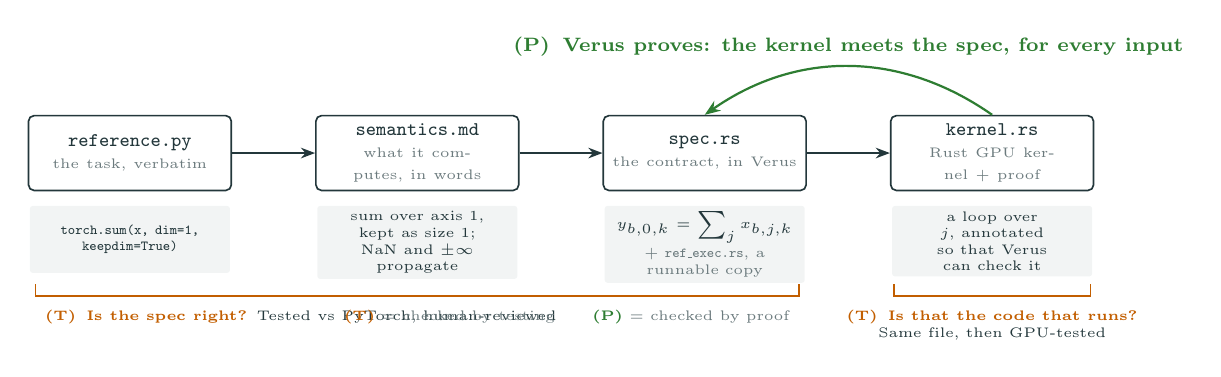
\begin{tikzpicture}[
    x=1mm, y=1mm,
    file/.style={draw=lgInk, line width=0.6pt, rounded corners=2pt, fill=white,
                 text width=24mm, align=center, inner sep=2.5pt, minimum height=9.5mm,
                 anchor=north, font=\scriptsize, text=lgInk},
    ex/.style={fill=lgWash, rounded corners=1pt, text width=24mm, align=center,
               font=\tiny, inner sep=2pt, minimum height=8.5mm, anchor=north, text=lgInk},
    fw/.style={-{Stealth[length=1.8mm]}, line width=0.7pt, draw=lgInk},
  ]
  \node[file] (f1) at (14.5,0)  {\code{\textbf{reference.py}}\\{\tiny\color{lgGrey}the task, verbatim}};
  \node[file] (f2) at (51,0)    {\code{\textbf{semantics.md}}\\{\tiny\color{lgGrey}what it computes, in words}};
  \node[file] (f3) at (87.5,0)  {\code{\textbf{spec.rs}}\\{\tiny\color{lgGrey}the contract, in Verus}};
  \node[file] (f4) at (124,0)   {\code{\textbf{kernel.rs}}\\{\tiny\color{lgGrey}Rust GPU kernel + proof}};
  \draw[fw] (f1.east) -- (f2.west);
  \draw[fw] (f2.east) -- (f3.west);
  \draw[fw] (f3.east) -- (f4.west);

  \node[ex] at (14.5,-11.5) {\code{torch.sum(x, dim=1,}\\\code{keepdim=True)}};
  \node[ex] at (51,-11.5)   {sum over axis 1, kept as size 1;\\NaN and $\pm\infty$ propagate};
  \node[ex] at (87.5,-11.5) {$y_{b,0,k} = \sum_{j} x_{b,j,k}$\\[1pt]{\color{lgGrey}+ \code{ref\_exec.rs}, a runnable copy}};
  \node[ex] at (124,-11.5)  {a loop over $j$, annotated\\so that Verus can check it};

  \draw[-{Stealth[length=2mm]}, line width=0.8pt, draw=lgGreen]
    (f4.north) to[bend right=35]
    node[above, font=\scriptsize\bfseries, text=lgGreen] {(P)\enspace Verus proves: the kernel meets the spec, for every input}
    (f3.north);

  % testing checks (T), bracketed under the files they tie together
  \draw[lgAccent, line width=0.6pt] (2.5,-21.5) -- ++(0,-1.5) -| (99.5,-21.5);
  \node[anchor=north west, font=\tiny, text=lgInk] at (2.5,-23.6)
    {{\color{lgAccent}\textbf{(T)\enspace Is the spec right?}}\enspace Tested vs PyTorch, human-reviewed};
  \draw[lgAccent, line width=0.6pt] (111.5,-21.5) -- ++(0,-1.5) -| (136.5,-21.5);
  \node[anchor=north, font=\tiny, text=lgInk, align=center] at (124,-23.6)
    {{\color{lgAccent}\textbf{(T)\enspace Is that the code that runs?}}\\Same file, then GPU-tested};
  \node[anchor=north east, font=\tiny, text=lgGrey] at (99.5,-23.6)
    {{\color{lgAccent}\textbf{(T)}} = checked by testing\qquad{\color{lgGreen}\textbf{(P)}} = checked by proof};
\end{tikzpicture}

\vspace{2pt}
{\scriptsize\hd{semantics.md records:}\enspace
\chip{Operator \& defaults} \chip{Dtypes} \chip{Layout} \chip{Preconditions}
\chip{Parameters \& state} \chip{Special values} \chip{Reduction order} \chip{Domains}\par}

\vfill
\begin{callout}[lgAccent]
\scriptsize\raggedright
\textbf{Special values:} corner cases such as NaN, $\pm\infty$ and $-0.0$, which KernelBench's random input
generator never produces.\quad
\textbf{Reduction order:} the order of the additions, which changes a float result.
\end{callout}
\vspace{4pt}

\note[itemize]{
\item \code{ref\_exec.rs} is an executable copy of the spec, used to test the spec on concrete inputs.
\item Each entry also has \code{adapter.py}, the glue that runs the kernel on the test inputs.
}
\end{frame}

% =====================================================================
\begin{frame}[t]{Humans define, agents scale\byanamul}

\begin{columns}[T]
\begin{column}{0.50\textwidth}
{\scriptsize\hd{100 KernelBench L1 tasks, grouped into 9 families}\par}
\vspace{4pt}
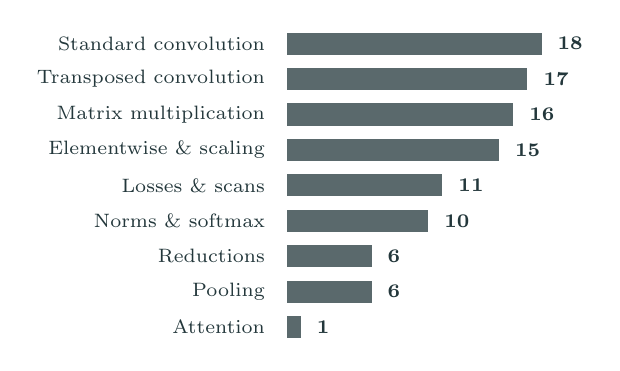
\begin{tikzpicture}[x=1mm, y=1mm]
  \foreach \name/\k [count=\i] in {
      Standard convolution/18, Transposed convolution/17, Matrix multiplication/16,
      Elementwise \& scaling/15, Losses \& scans/11, Norms \& softmax/10,
      Reductions/6, Pooling/6, Attention/1} {
    \node[anchor=east, font=\scriptsize, text=lgInk] at (30, -\i*4.5) {\name};
    \fill[lgInk!75] (31.5, -\i*4.5-1.4) rectangle ++(\k*1.8, 2.8);
    \node[anchor=west, font=\scriptsize\bfseries, text=lgInk] at (32.3+\k*1.8, -\i*4.5) {\k};
  }
\end{tikzpicture}
\end{column}

\begin{column}{0.46\textwidth}
\begin{actorbox}[lgAccent]
{\scriptsize\bfseries\color{lgAccent}Human defines}\par\vspace{5pt}
\scriptsize\raggedright
\stepline[lgAccent]{1}{Group the 100 tasks into families by shared structure.}
\stepline[lgAccent]{2}{Document each family: its characteristics and how to build it.}
\stepline[lgAccent]{3}{Verify one \emph{pilot} entry per family by hand.}
\end{actorbox}

{\centering
\tikz\draw[-{Stealth[length=2mm]}, line width=0.7pt, draw=lgGrey] (0,0) -- node[right, font=\tiny\itshape, text=lgGrey] {family note + pilot entry} (0,-0.45);\par}

\begin{actorbox}[lgInk]
{\scriptsize\bfseries\color{lgInk}Agents scale}\par\vspace{5pt}
\scriptsize\raggedright
Build every other task in the family, with the family note and the pilot entry as the reference
(next slide).
\end{actorbox}
\end{column}
\end{columns}

\vfill
\begin{callout}[lgAccent]
\scriptsize
\textbf{Why families.} Human effort grows with the number of families (9), not with the number of tasks (100).
\end{callout}
\vspace{4pt}

\end{frame}

% =====================================================================
\begin{frame}[t]{The construction loop\byanamul}

\vspace{-4pt}
\centering
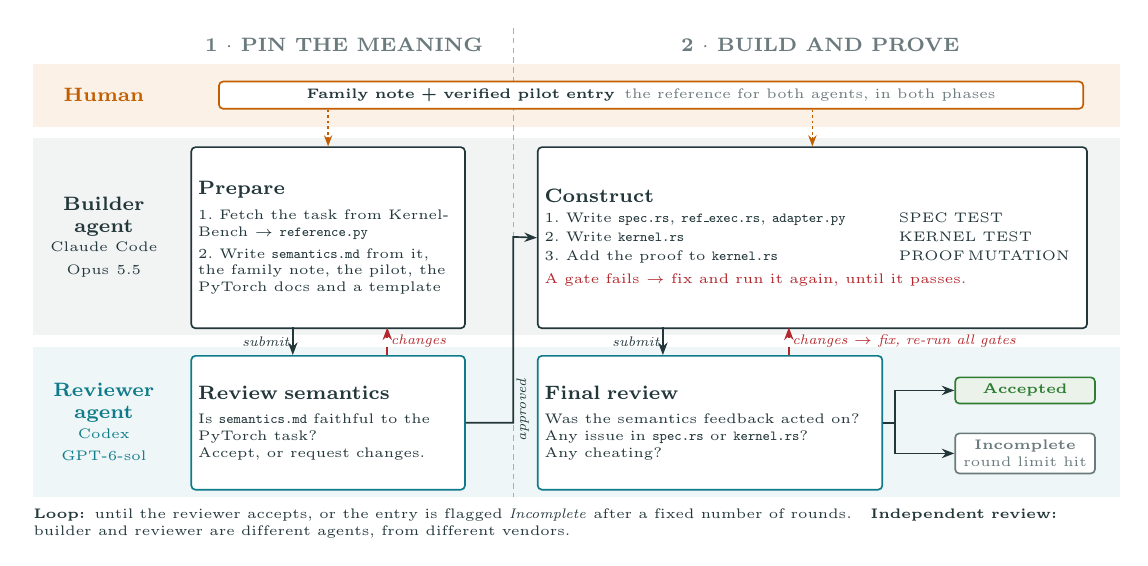
\begin{tikzpicture}[
    x=1mm, y=1mm,
    lane/.style={font=\scriptsize, align=center, text width=17mm},
    box/.style={draw, rounded corners=1.5pt, line width=0.6pt, font=\tiny, align=left, inner sep=2.5pt},
    bld/.style={box, draw=lgInk, fill=white, text=lgInk},
    rev/.style={box, draw=lgTeal, fill=white, text=lgInk},
    hum/.style={box, draw=lgAccent, fill=white, text=lgInk, align=center},
    fw/.style={-{Stealth[length=1.6mm]}, line width=0.6pt, draw=lgInk},
    bk/.style={-{Stealth[length=1.6mm]}, line width=0.6pt, draw=lgRed, dashed},
    rf/.style={-{Stealth[length=1.4mm]}, line width=0.6pt, draw=lgAccent, dash pattern=on 1pt off 1pt},
    el/.style={font=\tiny\itshape, inner sep=1pt},
    ph/.style={font=\scriptsize\bfseries, text=lgGrey},
  ]
  % lanes (total width 138 mm; text width is 140 mm)
  \fill[lgWashWarm] (0,0) rectangle (138,-8);
  \fill[lgWash]     (0,-9.5) rectangle (138,-34.5);
  \fill[lgTeal!7]   (0,-36) rectangle (138,-55);
  \node[lane, text=lgAccent] at (9,-4) {\textbf{Human}};
  \node[lane, text=lgInk]  at (9,-22) {\textbf{Builder agent}\\[1pt]{\tiny Claude Code\\Opus 5.5}};
  \node[lane, text=lgTeal] at (9,-45.5) {\textbf{Reviewer agent}\\[1pt]{\tiny Codex\\GPT-6-sol}};

  % phases
  \node[ph] at (39.5, 2.4) {1 $\cdot$ PIN THE MEANING};
  \node[ph] at (100, 2.4)  {2 $\cdot$ BUILD AND PROVE};
  \draw[lgGrey!60, line width=0.4pt, dash pattern=on 2pt off 1.5pt] (61, 4.5) -- (61, -55);

  % human
  \node[hum, text width=108mm] (h) at (78.5,-4)
    {\textbf{Family note + verified pilot entry}\enspace{\color{lgGrey}the reference for both agents, in both phases}};

  % builder
  \node[bld, text width=33mm, minimum height=23mm, anchor=north west] (p) at (20,-10.5)
    {{\scriptsize\bfseries Prepare}\\[3pt]
     1.\ Fetch the task from KernelBench $\to$ \code{reference.py}\\[2pt]
     2.\ Write \code{semantics.md} from it, the family note, the pilot, the PyTorch docs and a template};
  \node[bld, text width=68mm, minimum height=23mm, anchor=north west] (c) at (64,-10.5)
    {{\scriptsize\bfseries Construct}\\[2pt]
     \begin{tabular}{@{}p{43mm}@{\hspace{2mm}}l@{}}
       1.\ Write \code{spec.rs}, \code{ref\_exec.rs}, \code{adapter.py} & \gate{SPEC TEST} \\[1pt]
       2.\ Write \code{kernel.rs}                                        & \gate{KERNEL TEST} \\[1pt]
       3.\ Add the proof to \code{kernel.rs}                            & \gate{PROOF}\,\gate{MUTATION} \\
     \end{tabular}\\[2pt]
     {\color{lgRed}A gate fails $\to$ fix and run it again, until it passes.}};

  % reviewer
  \node[rev, text width=33mm, minimum height=17mm, anchor=north west] (r1) at (20,-37)
    {{\scriptsize\bfseries Review semantics}\\[3pt]
     Is \code{semantics.md} faithful to the PyTorch task?\\
     Accept, or request changes.};
  \node[rev, text width=42mm, minimum height=17mm, anchor=north west] (r2) at (64,-37)
    {{\scriptsize\bfseries Final review}\\[3pt]
     Was the semantics feedback acted on?\\
     Any issue in \code{spec.rs} or \code{kernel.rs}?\\
     Any cheating?};
  \node[box, draw=lgGreen, fill=lgGreen!10, text=lgGreen, align=center, text width=16mm] (acc) at (126,-41.5)
    {\textbf{Accepted}};
  \node[box, draw=lgGrey, fill=white, text=lgGrey, align=center, text width=16mm] (inc) at (126,-49.5)
    {\textbf{Incomplete}\\round limit hit};

  % human reference
  \draw[rf] (h.south -| p.north) -- (p.north);
  \draw[rf] (h.south -| c.north) -- (c.north);

  % phase 1 loop
  \draw[fw] (33,-33.5) -- node[el, left, text=lgInk] {submit} (33,-37);
  \draw[bk] (45,-37) -- node[el, right, text=lgRed] {changes} (45,-33.5);
  % phase 1 -> phase 2
  \draw[fw] (r1.east) -| (61,-22) -- (c.west);
  \node[el, rotate=90, anchor=north, text=lgInk] at (61,-44) {approved};

  % phase 2 loop
  \draw[fw] (80,-33.5) -- node[el, left, text=lgInk] {submit} (80,-37);
  \draw[bk] (96,-37) -- node[el, right, text=lgRed] {changes $\to$ fix, re-run all gates} (96,-33.5);
  \draw[fw] (r2.east) -- ++(1.5,0) |- (acc.west);
  \draw[fw] (r2.east) -- ++(1.5,0) |- (inc.west);

  % footer
  \node[anchor=north west, font=\tiny, text=lgInk, text width=136mm, align=left, inner sep=0pt] at (0,-56.5)
    {\textbf{Loop:} until the reviewer accepts, or the entry is flagged \emph{Incomplete} after a fixed number of rounds.\quad
     \textbf{Independent review:} builder and reviewer are different agents, from different vendors.};
\end{tikzpicture}

\note[itemize]{
\item Prepare, Construct and Review are three agent skills. Prepare and Construct run in the builder agent, Review in the reviewer agent.
\item The four green gates are explained on the next slide.
}
\end{frame}

% =====================================================================
\begin{frame}[t]{Task 47: End to End}

\vspace{-8pt}
\centering
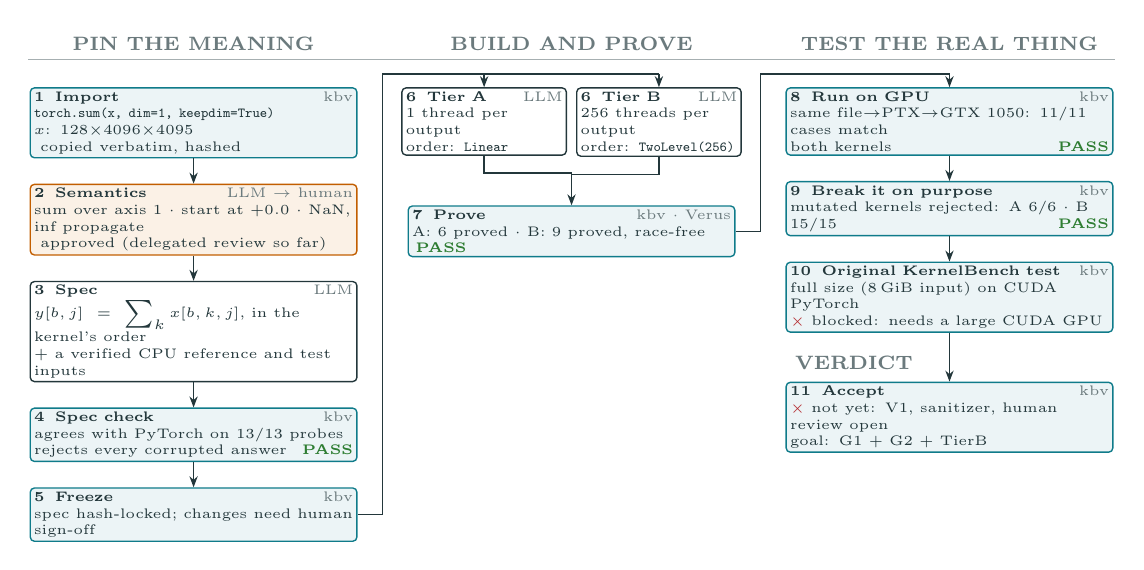
\begin{tikzpicture}[
    x=1mm, y=1mm,
    bx/.style={draw, rounded corners=1.5pt, line width=0.5pt, font=\tiny, align=left,
               text width=40.5mm, inner sep=1.4pt, anchor=north,
               execute at begin node={\hyphenpenalty=10000\exhyphenpenalty=10000}},
    ag/.style={bx, draw=lgInk, fill=white, text=lgInk},
    hv/.style={bx, draw=lgTeal, fill=lgTeal!8, text=lgInk},
    hu/.style={bx, draw=lgAccent, fill=lgWashWarm, text=lgInk},
    half/.style={text width=19.9mm},
    fw/.style={-{Stealth[length=1.4mm]}, line width=0.5pt, draw=lgInk},
    ph/.style={font=\scriptsize\bfseries, text=lgGrey, anchor=base},
    gap/.style={node distance=3.2mm},
  ]
  \def\ok{{\color{lgGreen}\checkmark}}
  \def\no{{\color{lgRed}$\boldsymbol{\times}$}}
  \def\pass{\hfill\mbox{\color{lgGreen}\textbf{\checkmark\,PASS}}}

  \node[ph] at (21, 1.2)  {PIN THE MEANING};
  \node[ph] at (69, 1.2)  {BUILD AND PROVE};
  \node[ph] at (117, 1.2) {TEST THE REAL THING};
  \draw[lgGrey!60, line width=0.4pt] (0, 0) -- (138, 0);

  % --- pin the meaning
  \node[hv] (s1) at (21, -3.5) {\textbf{1\enspace Import}\hfill{\color{lgGrey}kbv}\\
      \code{torch.sum(x, dim=1, keepdim=True)}\\ $x$: $128{\times}4096{\times}4095$\\
      \ok\ copied verbatim, hashed};
  \node[hu, gap, below=of s1] (s2) {\textbf{2\enspace Semantics}\hfill{\color{lgGrey}LLM $\to$ human}\\
      sum over axis 1 $\cdot$ start at $+0.0$ $\cdot$ NaN, inf propagate\\
      \ok\ approved (delegated review so far)};
  \node[ag, gap, below=of s2] (s3) {\textbf{3\enspace Spec}\hfill{\color{lgGrey}LLM}\\
      $y[b,j] = \sum_k x[b,k,j]$, in the kernel's order\\
      + a verified CPU reference and test inputs};
  \node[hv, gap, below=of s3] (s4) {\textbf{4\enspace Spec check}\hfill{\color{lgGrey}kbv}\\
      agrees with PyTorch on 13/13 probes\\
      rejects every corrupted answer\pass};
  \node[hv, gap, below=of s4] (s5) {\textbf{5\enspace Freeze}\hfill{\color{lgGrey}kbv}\\
      spec hash-locked; changes need human sign-off};
  \draw[fw] (s1) -- (s2); \draw[fw] (s2) -- (s3); \draw[fw] (s3) -- (s4); \draw[fw] (s4) -- (s5);

  % --- build and prove
  \node[ag, half] (s6a) at (57.9, -3.5) {\textbf{6\enspace Tier A}\hfill{\color{lgGrey}LLM}\\
      1 thread per output\\ order: \code{Linear}};
  \node[ag, half] (s6b) at (80.1, -3.5) {\textbf{6\enspace Tier B}\hfill{\color{lgGrey}LLM}\\
      256 threads per output\\ order: \code{TwoLevel(256)}};
  \path (s6a.south) -- coordinate (mid) (s6b.south);
  \node[hv, anchor=north] (s7) at (69, -18.5) {\textbf{7\enspace Prove}\hfill{\color{lgGrey}kbv $\cdot$ Verus}\\
      A: 6 proved $\cdot$ B: 9 proved, race-free\pass};
  \draw[fw] (s6a.south) |- ++(11.1, -2.2) -| (s7.north);
  \draw[line width=0.5pt, draw=lgInk] (s6b.south) |- ++(-11.1, -2.2);

  % 5 -> 6: out of the right side of 5, up the gutter, fork into both kernels
  \draw[line width=0.5pt, draw=lgInk] (s5.east) -- (45, 0 |- s5.east) -- (45, -1.8) -| (69, -1.8);
  \draw[fw] (57.9, -1.8) -- (s6a.north);
  \draw[fw] (80.1, -1.8) -- (s6b.north);
  \draw[line width=0.5pt, draw=lgInk] (57.9, -1.8) -- (80.1, -1.8);

  % --- test the real thing
  \node[hv] (s8) at (117, -3.5) {\textbf{8\enspace Run on GPU}\hfill{\color{lgGrey}kbv}\\
      same file${\to}$PTX${\to}$GTX 1050: 11/11 cases match\\
      both kernels\pass};
  \node[hv, gap, below=of s8] (s9) {\textbf{9\enspace Break it on purpose}\hfill{\color{lgGrey}kbv}\\
      mutated kernels rejected: A 6/6 $\cdot$ B 15/15\pass};
  \node[hv, gap, below=of s9] (s10) {\textbf{10\enspace Original KernelBench test}\hfill{\color{lgGrey}kbv}\\
      full size (8\,GiB input) on CUDA PyTorch\\
      \no\ blocked: needs a large CUDA GPU};
  \node[ph, anchor=base west] (vh) at ($(s10.south west) + (0, -4.6)$) {VERDICT};
  \node[hv, anchor=north] (s11) at ($(s10.south) + (0, -6.2)$) {\textbf{11\enspace Accept}\hfill{\color{lgGrey}kbv}\\
      \no\ not yet: V1, sanitizer, human review open\\
      goal: G1 + G2 + TierB};
  \draw[fw] (s8) -- (s9); \draw[fw] (s9) -- (s10); \draw[fw] (s10) -- (s11);

  % 7 -> 8: out of the right side of 7, up the gutter, into the top of 8
  \draw[fw] (s7.east) -- (93, 0 |- s7.east) -- (93, -1.8) -| (s8.north);
\end{tikzpicture}

\note[itemize]{
\item Step 4: ``13/13 probes'' is V2 (6 exact-arithmetic cases and 7 edge-case rules). ``Rejects every corrupted answer'' is V3.
\item Step 7: ``6 proved'' and ``9 proved'' are Verus proof obligations for the Tier A and Tier B kernels. Tier B's barrier uniformity comes from the lint, not the proof.
\item Step 9: these are program mutants, meaning deliberately broken kernels, as opposed to step 4's corrupted outputs.
}
\end{frame}

% =====================================================================
\begin{frame}[t]{Four gates: why trust an entry\byanamul}

{\scriptsize
Inside \emph{Construct}, every entry must pass four automatic gates run by the harness.
A failed gate goes back to the builder, which fixes the files and runs the gate again.\par
}

\vspace{4pt}
{\scriptsize
\setlength{\tabcolsep}{4pt}
\renewcommand{\arraystretch}{1.3}
\begin{tabular}{@{}p{21mm} p{30mm} p{56mm} p{22mm}@{}}
\toprule
\textbf{Gate} & \textbf{Question} & \textbf{How} & \textbf{Passes when} \\
\midrule
\raggedright \anum{1}\ \textbf{Spec test}\newline\pill{lgGrey}{TEST}
  & \raggedright Does \code{spec.rs} say what PyTorch computes?
  & \raggedright Verus checks the spec on concrete cases.
    \good{\textbf{Positive:}} small-integer inputs (exact output), plus corner and
    tolerance cases from \code{semantics.md}.
    \bad{\textbf{Negative:}} mutated outputs.
  & \raggedright every positive holds, every negative is rejected \tabularnewline
\raggedright \anum{2}\ \textbf{Kernel test}\newline\pill{lgGrey}{TEST}
  & \raggedright Does \code{kernel.rs} compute the right numbers?
  & \raggedright Run it on KernelBench's own test inputs and compare with PyTorch.
  & \raggedright results match, within tolerance \tabularnewline
\raggedright \anum{3}\ \textbf{Proof}\newline\pill{lgGreen}{PROOF}
  & \raggedright Does \code{kernel.rs} meet \code{spec.rs} for \emph{every} input?
  & \raggedright Verus checks the proof in \code{kernel.rs} against the spec.
  & \raggedright Verus accepts \tabularnewline
\raggedright \anum{4}\ \textbf{Mutation}\newline\pill{lgGreen}{PROOF}
  & \raggedright Is the proof meaningful, not vacuous?
  & \raggedright Break \code{kernel.rs} on purpose (mutants) and run Verus again.
  & \raggedright every mutant is rejected \tabularnewline
\bottomrule
\end{tabular}
}

\vfill
\begin{callout}[lgAccent]
\scriptsize\raggedright
\textbf{Together.} Tests tie the spec to PyTorch on known cases; the proof then covers every input
against that spec; mutation shows that the proof actually constrains the kernel.
\end{callout}
\vspace{4pt}

\end{frame}

% =====================================================================
\begin{frame}[t]{Evaluating LLMs: three levels of help\byanamul}

{\scriptsize
An entry is a chain of files. Each evaluation task gives the LLM one file and asks it to produce the spec and
the kernel.\par
}

\vspace{10pt}
\centering
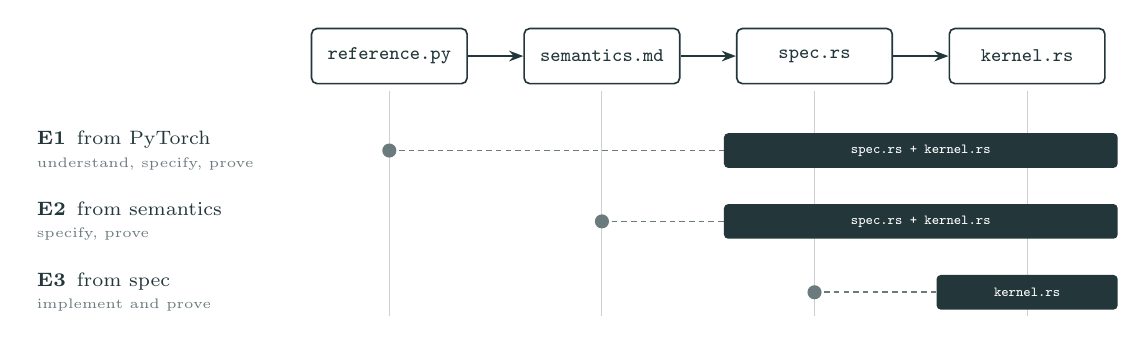
\begin{tikzpicture}[
    x=1mm, y=1mm,
    file/.style={draw=lgInk, line width=0.6pt, rounded corners=2pt, fill=white,
                 text width=18mm, align=center, inner sep=2.5pt, minimum height=7mm,
                 font=\scriptsize\ttfamily\bfseries, text=lgInk},
    fw/.style={-{Stealth[length=1.8mm]}, line width=0.7pt, draw=lgInk},
    rl/.style={anchor=west, align=left, font=\scriptsize, text=lgInk},
    given/.style={circle, fill=lgGrey, inner sep=1.8pt},
    skip/.style={lgGrey, line width=0.6pt, dash pattern=on 2pt off 1.5pt},
    prod/.style={rounded corners=1.5pt, fill=lgInk, text=white, font=\tiny\ttfamily\bfseries,
                 minimum height=4.4mm, inner sep=1pt},
  ]
  % file columns at x = 46, 73, 100, 127; each box is 23 mm wide
  \def\ya{-12}\def\yb{-21}\def\yc{-30}
  \node[file] (a) at (46,0)  {reference.py};
  \node[file] (b) at (73,0)  {semantics.md};
  \node[file] (c) at (100,0) {spec.rs};
  \node[file] (d) at (127,0) {kernel.rs};
  \draw[fw] (a) -- (b);
  \draw[fw] (b) -- (c);
  \draw[fw] (c) -- (d);
  \foreach \x in {46,73,100,127} \draw[lgGrey!35, line width=0.4pt] (\x,-4.5) -- (\x,-33);

  \node[rl] at (0,\ya) {\textbf{E1}\enspace from PyTorch\\{\tiny\color{lgGrey}understand, specify, prove}};
  \draw[skip] (46,\ya) -- (88.5,\ya);
  \node[given] at (46,\ya) {};
  \node[prod, minimum width=50mm] at (113.5,\ya) {spec.rs + kernel.rs};

  \node[rl] at (0,\yb) {\textbf{E2}\enspace from semantics\\{\tiny\color{lgGrey}specify, prove}};
  \draw[skip] (73,\yb) -- (88.5,\yb);
  \node[given] at (73,\yb) {};
  \node[prod, minimum width=50mm] at (113.5,\yb) {spec.rs + kernel.rs};

  \node[rl] at (0,\yc) {\textbf{E3}\enspace from spec\\{\tiny\color{lgGrey}implement and prove}};
  \draw[skip] (100,\yc) -- (115.5,\yc);
  \node[given] at (100,\yc) {};
  \node[prod, minimum width=23mm] at (127,\yc) {kernel.rs};
\end{tikzpicture}

\vspace{6pt}
{\tiny\color{lgInk}
\tikz[baseline=-0.6ex]\node[circle, fill=lgGrey, inner sep=1.8pt] {};\ given to the LLM
\qquad
\tikz[baseline=-0.6ex]\fill[lgInk, rounded corners=0.8pt] (0,-0.9mm) rectangle (6mm,0.9mm);\ produced by the LLM, then checked by the harness gates\par}

\vfill
\begin{callout}[lgAccent]
\scriptsize\raggedright
\textbf{Why three levels.} Comparing E1, E2 and E3 shows where an LLM breaks down: understanding the
PyTorch task, writing a faithful spec, or building a kernel that Verus accepts.
\end{callout}
\vspace{4pt}

\end{frame}

% =====================================================================
\begin{frame}{Current Landscape}

\centering
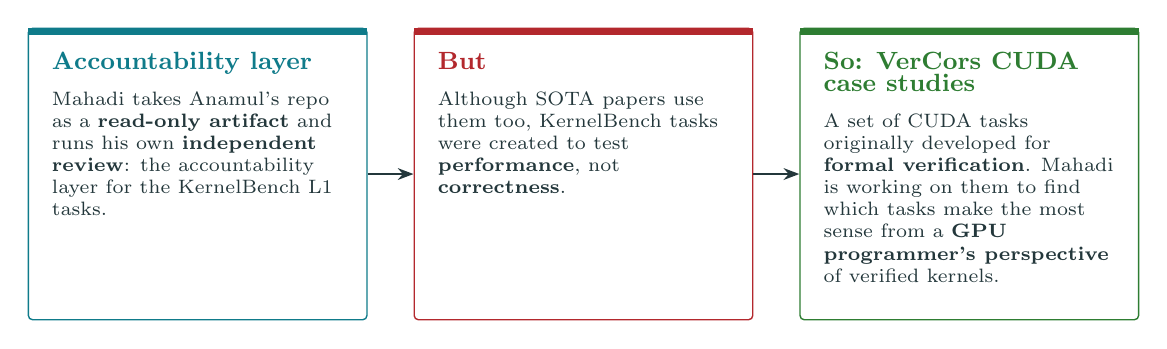
\begin{tikzpicture}[
    x=1mm, y=1mm,
    card/.style={draw, line width=0.5pt, rounded corners=1.5pt, fill=white,
                 inner sep=3mm, anchor=north, font=\scriptsize, text=lgInk,
                 execute at begin node={\hyphenpenalty=10000\exhyphenpenalty=10000}},
  ]
  \node[card, draw=lgTeal] (a) at (21,0)
    {\begin{minipage}[t][31mm][t]{37mm}\raggedright
     {\small\bfseries\color{lgTeal}Accountability layer}\\[5pt]
     Mahadi takes Anamul's repo as a \textbf{read-only artifact} and runs his own
     \textbf{independent review}: the accountability layer for the KernelBench L1 tasks.
     \end{minipage}};
  \node[card, draw=lgRed] (b) at (70,0)
    {\begin{minipage}[t][31mm][t]{37mm}\raggedright
     {\small\bfseries\color{lgRed}But}\\[5pt]
     Although SOTA papers use them too, KernelBench tasks were created to test
     \textbf{performance}, not \textbf{correctness}.
     \end{minipage}};
  \node[card, draw=lgGreen] (c) at (119,0)
    {\begin{minipage}[t][31mm][t]{37mm}\raggedright
     {\small\bfseries\color{lgGreen}So: VerCors CUDA case studies}\\[5pt]
     A set of CUDA tasks originally developed for \textbf{formal verification}.
     Mahadi is working on them to find which tasks make the most sense from a
     \textbf{GPU programmer's perspective} of verified kernels.
     \end{minipage}};
  \foreach \n/\col in {a/lgTeal, b/lgRed, c/lgGreen}
    \fill[\col] ([xshift=0.25pt]\n.north west) rectangle ([xshift=-0.25pt, yshift=-0.9mm]\n.north east);
  \draw[flow] (a.east) -- (b.west);
  \draw[flow] (b.east) -- (c.west);
\end{tikzpicture}

\end{frame}

% =====================================================================
\begin{frame}[fragile]{Publication Target}

{\scriptsize
Reframing the paper for the following venues:\par
}

\vspace{0pt}
{\scriptsize
\renewcommand{\arraystretch}{1.15}
\begin{tabular}{@{}l l l p{59mm} l@{}}
\toprule
 & \textbf{Venue} & \textbf{Deadline} & \textbf{Focus} & \textbf{Confidence} \\
\midrule
\pill{lgAccent}{TARGET}
  & \hd{LLM4Code @ ICSE 2027} & 13 Nov 2026 & \raggedright Non-archival option \textcolor{lgGrey}{(tentative)}
  & \good{\textbf{High}} \tabularnewline
\midrule
\pill{lgGrey}{LATER TARGET}
  & \hd{CAV 2027}   & 20 Jan 2027 & \raggedright \textbf{Verification.} Propose an agent-based verification technique: the
                                    block-synchronous GPU model, its soundness argument, and the order library.
  & \textcolor{lgAccent}{\textbf{Medium}} \tabularnewline
\pill{lgGrey}{LATER TARGET}
  & \hd{ISSTA 2027} & 11 Jan 2027 & \raggedright \textbf{Testing.} How weak KernelBench's oracle is, and how well spec
                                    validation catches defects.
  & \textcolor{lgAccent}{\textbf{Medium}} \tabularnewline
\bottomrule
\end{tabular}
}

\vspace{10pt}
{\scriptsize
\renewcommand{\arraystretch}{1.3}
\begin{tabular}{@{}l l l@{}}
\toprule
\textbf{Criteria} & \multicolumn{2}{l}{\textbf{Confidence}} \\
\midrule
Spec faithfulness & \multicolumn{2}{l}{\good{\textbf{High}}} \\
Technical rigor   & \bad{\textbf{Low}} (Nov) & \textcolor{lgAccent}{\textbf{Mid}} (Jan) \\
\bottomrule
\end{tabular}
}

\end{frame}

% =====================================================================
\begin{frame}{Review of the current dataset}

\begin{callout}[lgAccent]
\scriptsize\raggedright
\textbf{Technical rigor} is what Mahadi thinks the current dataset lacks, for example:
\setlength\leftmargini{1.2em}
\begin{itemize}\setlength\itemsep{1pt}
  \item Verus does not support float arithmetic, but Mahadi finds that Anamul's current PoC replaces
        float addition with a trusted \code{\#[verifier::external\_body]} function.
  \item SOTA papers like \emph{Kuiper} do not do this; rather, they show the approximation explicitly.
  \item The dataset's Rust code is generated by LLMs without the frameworks real GPU programmers would use in future work,
        i.e.\ \code{cuda-oxide} or \code{cuTile-Rust}.
  \item In Mahadi's own findings, using \code{cuda-oxide} or \code{cuTile-Rust} with in-place Verus
        annotations, which real GPU communities would actually use, is more time-consuming and less
        likely to fit the Nov deadline.
\end{itemize}
\end{callout}

\vspace{6pt}
\begin{tcolorbox}[enhanced, colback=lgGreen!6, colframe=lgGreen,
  boxrule=0.1pt, leftrule=2.5pt, arc=1.5pt,
  left=6pt, right=6pt, top=4pt, bottom=4pt, boxsep=0pt]
\scriptsize\raggedright
\textbf{\color{lgGreen}Counter-argument.} These are engineering nitpicks that would not matter significantly.
The pipeline does the intended job, and it is better to focus on the research contributions instead.
\end{tcolorbox}

\end{frame}

% =====================================================================
\begin{frame}{Blockers and Literature}

\setlength\leftmargini{1.1em}
\begin{columns}[T]
\begin{column}{0.47\textwidth}
\begin{codebox}[lgRed]{Blockers}
\scriptsize\raggedright
\begin{itemize}\setlength\itemsep{3pt}
  \item Anamul has a GTX 1050 with 2\,GB VRAM, which is insufficient for many KernelBench L1 tasks.
  \item Mahadi got access to an RTX 3070 machine a couple of days ago. Claude estimates that
        about 60 of the 100 L1 tasks can be tested on it.
  \item \textbf{Ask:} access to a modern Nvidia GPU with 24\,GB VRAM, like an RTX 4090.
\end{itemize}
\end{codebox}
\end{column}

\begin{column}{0.47\textwidth}
\begin{codebox}[lgTeal]{Literature}
\scriptsize\raggedright
\begin{itemize}\setlength\itemsep{3pt}
  \item \emph{Kuiper: GPU Kernel Verification in Pulse} does almost the same work we are doing,
        so their dataset is helpful to cross-check against our Verus port.
  \item \emph{ProofWright: Towards Agentic Formal Verification of CUDA} claims it will open-source
        its artifact MLRocq, which converts PyTorch $\to$ Rocq ``deterministically'', but has not yet.
        Early access would potentially make our work easier and give another base to cross-check against.
\end{itemize}
\end{codebox}
\end{column}
\end{columns}

\end{frame}

% <<INSERT NEW SLIDES ABOVE THIS LINE>>
\end{document}
